\begin{figure}[H]
\centering
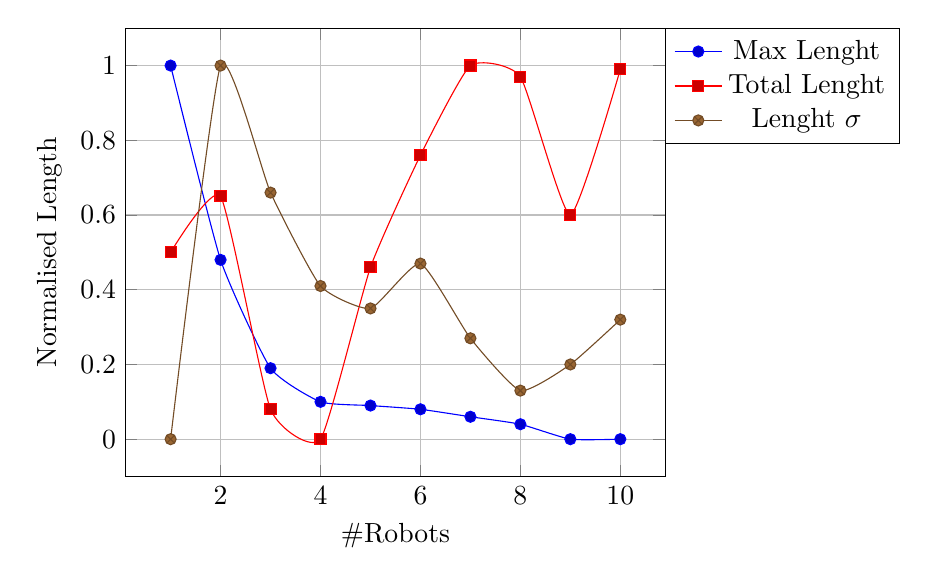
\begin{tikzpicture}
	\begin{axis}[
%		height=9cm,
%		width=9cm,
		grid=major,
                legend style = {at={(1,1)}, anchor=north west},
		xlabel=\#Robots,
		ylabel=Normalised Length,
		smooth,
		tension=0.3
	]

	\addplot coordinates {
(1, 1.00)
(2, 0.48)
(3, 0.19)
(4, 0.10)
(5, 0.09)
(6, 0.08)
(7, 0.06)
(8, 0.04)
(9, 0.00)
(10, 0.00)
	};
	\addlegendentry{Max Lenght}

	\addplot coordinates {
(1, 0.50)
(2, 0.65)
(3, 0.08)
(4, 0.00)
(5, 0.46)
(6, 0.76)
(7, 1.00)
(8, 0.97)
(9, 0.60)
(10, 0.99)
	};
	\addlegendentry{Total Lenght}

	\addplot coordinates {
(1, 0.00)
(2, 1.00)
(3, 0.66)
(4, 0.41)
(5, 0.35)
(6, 0.47)
(7, 0.27)
(8, 0.13)
(9, 0.20)
(10, 0.32)
	};
	\addlegendentry{Lenght $\sigma$}
	\end{axis}
\end{tikzpicture}
\caption{Variation of the performance indexes increasing the number of robots, for the 15x15 grid using the LRTA* algorithm}
\end{figure}